\documentclass[review]{elsarticle}

\usepackage{lineno,hyperref}
\modulolinenumbers[5]
\usepackage{booktabs}
\usepackage{graphicx}
\usepackage{float}
\graphicspath{ {./images/} }
\usepackage{adjustbox}

\usepackage{threeparttable}
\usepackage{amsmath}

\journal{International Journal of Forecasting}

%%%%%%%%%%%%%%%%%%%%%%%
%% Elsevier bibliography styles
%%%%%%%%%%%%%%%%%%%%%%%
%% To change the style, put a % in front of the second line of the current style and
%% remove the % from the second line of the style you would like to use.
%%%%%%%%%%%%%%%%%%%%%%%

%% Numbered
%\bibliographystyle{model1-num-names}

%% Numbered without titles
%\bibliographystyle{model1a-num-names}

%% Harvard
%\bibliographystyle{model2-names.bst}\biboptions{authoryear}

%% Vancouver numbered
%\usepackage{numcompress}\bibliographystyle{model3-num-names}

%% Vancouver name/year
%\usepackage{numcompress}\bibliographystyle{model4-names}\biboptions{authoryear}

%% APA style
%\bibliographystyle{model5-names}\biboptions{authoryear}

%% AMA style
%\usepackage{numcompress}\bibliographystyle{model6-num-names}

%% `Elsevier LaTeX' style
\bibliographystyle{elsarticle-num}
%%%%%%%%%%%%%%%%%%%%%%%

\begin{document}

  \begin{frontmatter}

    \title{A novel interval electricity price forecasting using deep residual neural networks}
    % \tnotetext[mytitlenote]{Fully documented templates are available in the elsarticle package on \href{http://www.ctan.org/tex-archive/macros/latex/contrib/elsarticle}{CTAN}.}

    %% Group authors per affiliation:
    % \author{Pornchai Chaweewat\fnref{myfootnote}}
    \author{Pornchai Chaweewat\fnref{myfootnote}}
    \author{J G singh\fnref{myfootnote2}}

    \address{Department of Energy, Environmental and Climate Change, School of Environmental, Resource and Development, Asian Institute of Thechnology, Thailand}
    \fntext[myfootnote]{email: chaweewat.p@gmail.com}
    \fntext[myfootnote2]{email: jgsingj@ait.ac.th}

    % %% or include affiliations in footnotes:
    % \author[mymainaddress,mysecondaryaddress]{Elsevier Inc}
    % \ead[url]{www.elsevier.com}
    %
    % \author[mysecondaryaddress]{Global Customer Service\corref{mycorrespondingauthor}}
    % \cortext[mycorrespondingauthor]{Corresponding author}
    % \ead{support@elsevier.com}
    %
    % \address[mymainaddress]{1600 John F Kennedy Boulevard, Philadelphia}
    % \address[mysecondaryaddress]{360 Park Avenue South, New York}

    \begin{abstract}
      % (What we do?)
      This paper proposed a novel electricity price forecasting method based on a novel Deep Residual Neural Network (Deep ResNet) for probabilistic electricity price forecasting under spike price environment.

      % (Why I do this?)
      The modern electricity price became more fluctuated and generally unanticipated spike price.
      The use of prediction interval or probabilistic forecasting was interested due to it help market participants to submit effective bid with low risks.

      % (How I do this?)
      A proposed new model was developed from Deep ResNet approach which it capable of spike price and price value prediction.
      The proposed Deep ResNet was consisting of two network layers.
      First neural network laver was spike prediction.
      The output of second neural networks layer formulated interval price forecasting by two methods; quantile regression and mean and varience estimation method.
      The proposed forecasting models was demonstrated with GEFCom2014 dataset where the dataset was consisting of 15 tasks for electricity price forecasting where high and spike price were included.
      The results were compared with benchmarkes provided by GEFCom2014, linear regression and multilayer perceptron network (MLP) methods.

      % (What is the result?)
      The performances of forecasting models were evaluated in term of accuracy and reliablity metrics by Pinball Loss Function and Coverage Width-baed Criterion (CWC), respectively.
      The significant outcome of this paper was forecasting method cooperated with spike price prediction imporved the forecasting's performance in term of quaility and quantity.
      Moreover, increasing in confidence level could generates higher CWC values and represent high reliability's satification.
    \end{abstract}

    \begin{keyword}
      ResNet, GEFCom2014, interval forecasting, quantile regression, mean and varience estimation
    \end{keyword}

  \end{frontmatter}

  \linenumbers

  \section{Introduction}

    Since the transformation of the deregulation of modern power systems, electricty price forecasting has become more important process to energy market's participants at planning and operation levels.
    As a result of higher number of fluctuated electricity price as well as the number of the spike price occurences.
    The occurrences of spike price can cause financial damage to both customers and producers.
    The spike prices can be reach several times to thousand times of the normal price.
    Spike price appears due to increasing intermittent electricity production makes electricity prices more volatile, with spikes appearing either as very high prices (due to sudden lack of available generation) or as negative prices (due to excess of renewable generation).
    Several evidences shows that the spike prices are around 100$\$$/MWhr may simply resulted from normal congestion or unexpected overload, while spike price around $\$$500/MWhr led by lacking of reserve.
    This case the day ahead clearing price was the dominant feature what indicate insufficient reserve. The spike price aboved $\$$1,000/MWhr should be the consequence of the outage or breakdown of the generation or transmission system.
    Such outage or breakdown many could came from many factors, like weather, load profile, etc  \cite{He2016}.
    \cite{SINGHAL2011550} provided fundamental reasons of spike price which are volatility of fuel price, load uncertainty, fluctuation in hydroelectricity production, generation outage, transmission congestion, behavior of market participation and market manipulation.
    \cite{GONZALEZSOTRES2017338} studied on technique and economical of on centralized voltage control with high PV penetration in Portuguese network.
    These results illustrated that improvement in both forecasting tools and communication systems have significant impact on dedicate resources and voltage control.

    % (talk about point of forecating, 1 method, 2 measurement, 3 problems)
    Over the past few decades, many powerful forecasting algorithms have been developed (for a recent comprehensive review, see \cite{Weron2014}).
    The majority of emprical studies was on point forecasting (or call expected value of the spot price).

    % (mention about problems of poing of forecasting, introduct to interval forecasting)
    The conventional point predictions produced no information about the sampling erros and the predicition accuracy.
    This lead to confidence intervals (CIs) and prediction intervals (PIs).
    CIs and PIs were two well-know toosl for quantifying and representing the uncertainty of predicitons.
    In literature, several methods have been proposed for construction of PIs and CIs assessment.
    Lower Upper Bounds Estimation (LUBE) method were formulated using mean and varience estimation which was proposed in \cite{Khosravi2011}.
    In addition, delta technique for PI construction was presented in \cite{KhosraviA2010}.

    % (mention on used of deep residual neural network and why we use this method)
    In computaional intelligent world, Deep Residual Neural Network (Deep ResNet) was modified from deep Feed Forward Neural Networks (FFNNs) with extra connections (or called skip connections), passing input from one layer to a late layer as well as the next layer as shown in figure~\ref{Fig:Basic_DRNN}.
    Deep ResNet was widely used in computer vision and pattern reconigtion.
    There were few used on deep residual neural network in forecasting applications.

    \begin{figure}[H]
      \centering
      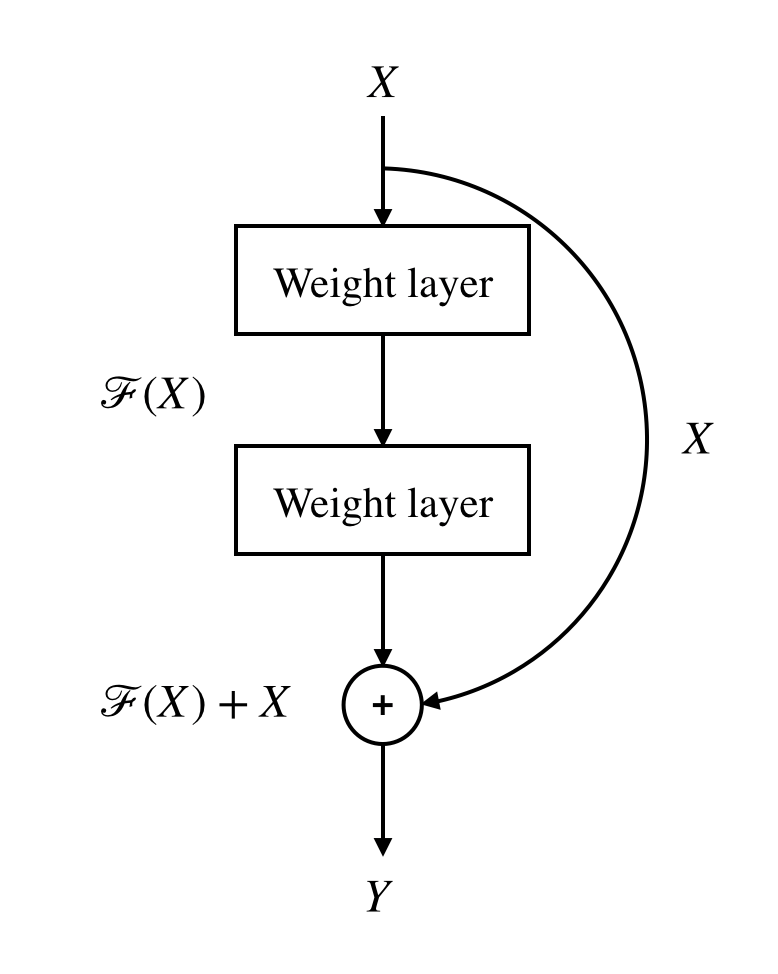
\includegraphics[width=5cm]{basic_DRNN}
      \caption{Basis concept of Residual Neural Network (ResNet)}
      \label{Fig:Basic_DRNN}
    \end{figure}


    % (proposal)
    Therefore, this paper seek to apply Deep ResNet in electricity price forecasting.
    The performance results of the Deep ResNet forecasting model were also compared with linear regression and MLP techniques.

    The novelty of this study is twofold.
    First, ResNet is first used in field of electricty price forecasting. Using this approach, the probabilistic electricity price forecasting can sastified both accuracy and reliability aspects.
    Second, CWC are used to evalueate interval electricity price forecasting.

    % The novelty of this study is threefold.
    % First, customer behaviors are integrated into the framework.
    % Each customer is handled individually, and the work shift constraint is considered.
    % Second, a game-theoretic approach to simulate the interaction between the utility and customers is proposed.
    % Using this approach, both optimal TOU pricing and demand response can be achieved simultaneously in the Nash-equilibrium, and the conflicting economic interests of the utility and customers can be captured clearly.
    % Third, different kinds of scenarios are investigated in case studies, which indicate that profitable results can be achieved for both sides and provide meaningful managerial insights for the practi- tioners.
    % The main findings in this study are summarized as follows.
    % (i) A good TOU price can be obtained by the game-theoretic model with the consideration of customer behaviors to create a win-win situation for the utility and customers.
    % (ii) The utility can control the interrelationship between two sides to improve its own profit. Meanwhile, attentions must be paid to the customer's credibility.
    % (iii) The customers are segregated naturally when facing the opportunity of TOU program. Therefore, the utility only need focus on the customer with a small penalty factor and a large auxiliary coefficient.
    % In fact, a small portion of customers joining the TOU program can also lead to a large improvement in utility's profit.
    % (iv) The profit of utility from the launch of TOU program is mainly affected by the expected values ofthe parameters on the client side, while it

    % (structure)
    The remainder of the paper is organized as follows.
    First, the problem formulation is presented in brief in section 2.
    The, the main features of the ANN algorithm are presented.
    Next, the results after prediction in different cases of proposed method  are discussed in section 4.
    Finally, conclusions are drawn in the last section of this paper.

  \section{Problem formulation}
    This section will descript construction of two proposed method; MLP and Deep ResNet model.
    The MPL model will represent electricity price forecasting without spike price prediction (see related work in \cite{Dudek2016}) and the Deep ResNet model will represent electricity price forecasting with spike price prediction in the model.
    Both model will generate upper and lower bounds with respect to given confidence levels (5$\%$, 10$\%$, 15$\%$, 20$\%$, and 25$\%$).
    The upper and lower bound will generate using quantile regression and mean-varience estimation metod.

    \subsection{Proposed Deep ResNet on interval forecasting}
      As mention eariler, this paper develop a novel Deep ResNet with spike price occurance and price  value prediction.
      The forecasted total load and zonal load (provided in GEFCom2014) and

      \begin{figure}[H]
        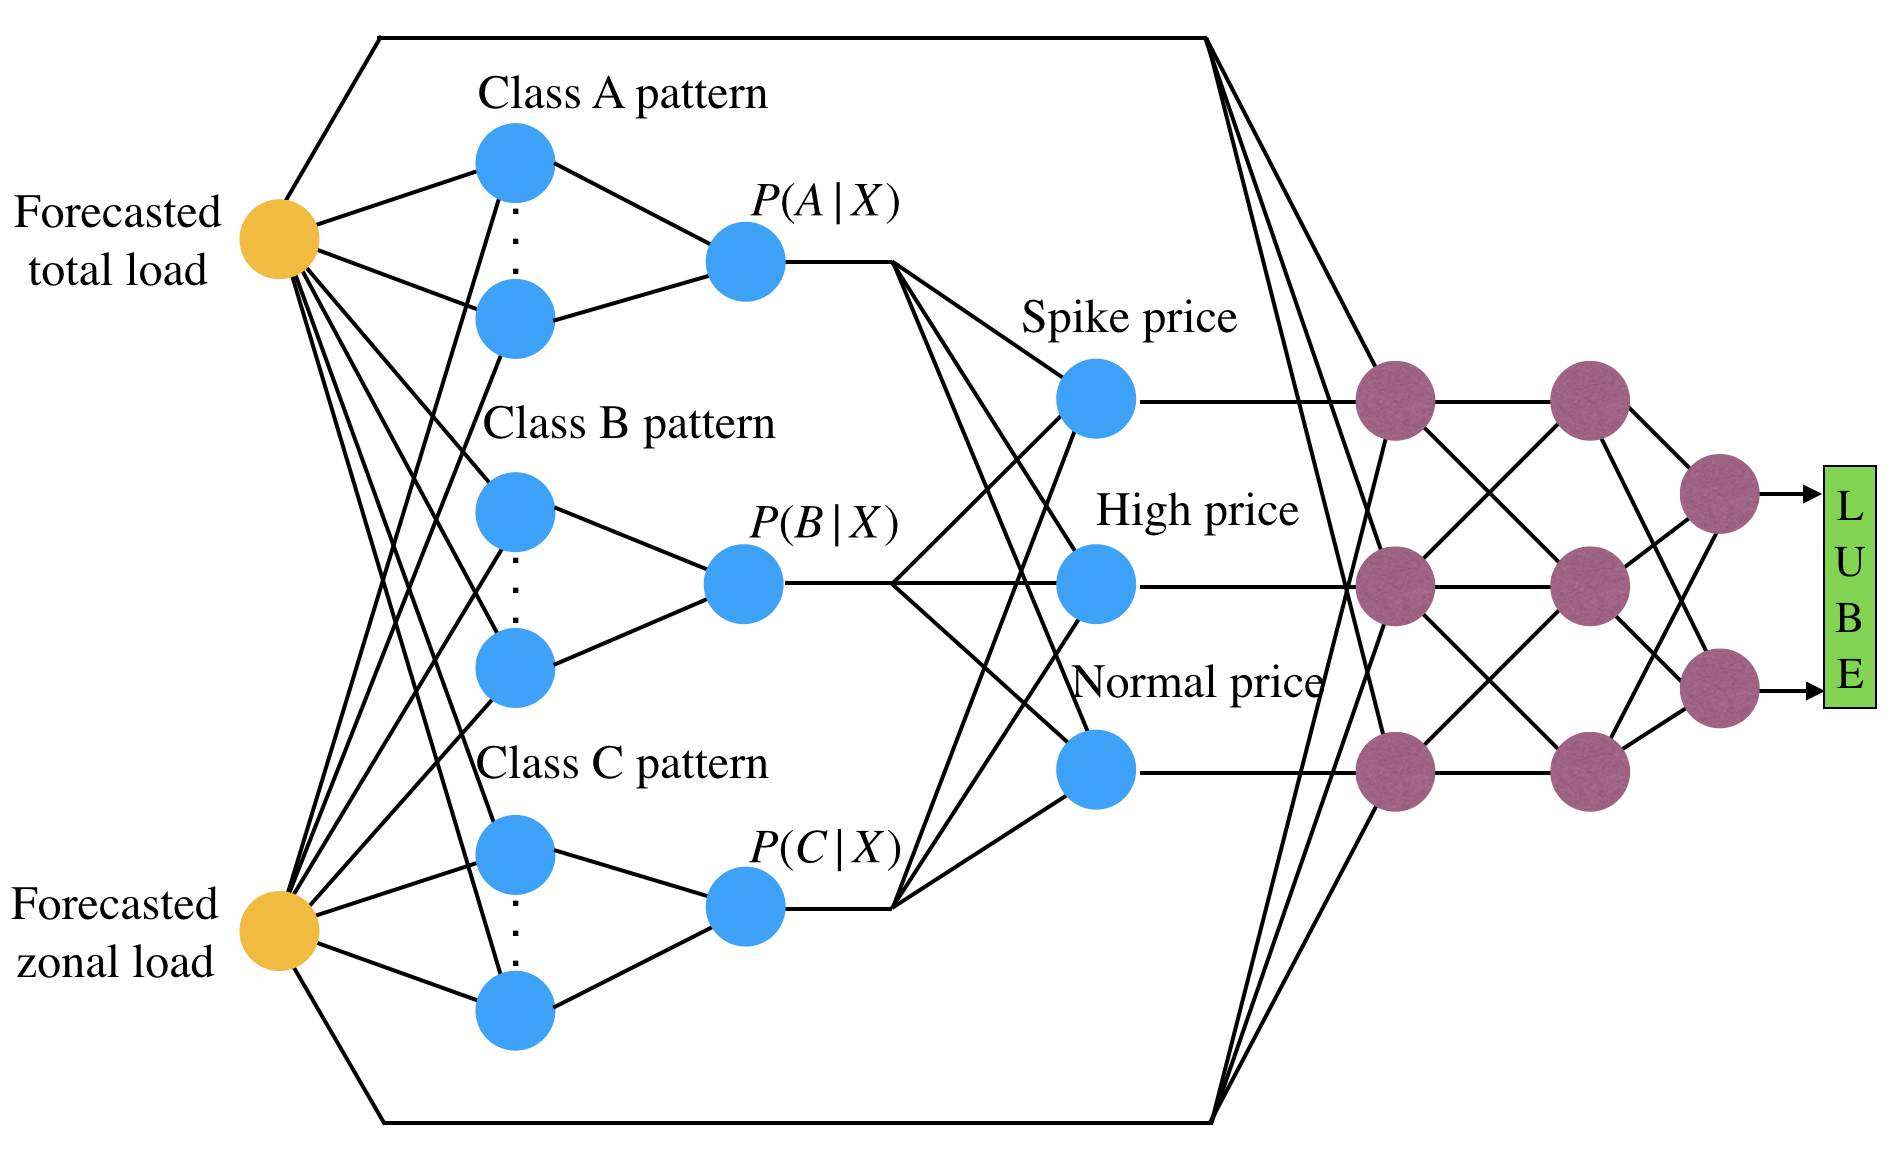
\includegraphics[width=12cm]{proposed_PDRNN}
        \caption{Proposed probabilistic Deep ResNet}
        \label{Fig:proposed_PDRNN}
        \centering
      \end{figure}

      The interval forecasting is formulated from two methods; lower and upper quantile regression, and mean and varianece estimation.
      \begin{figure}[H]
        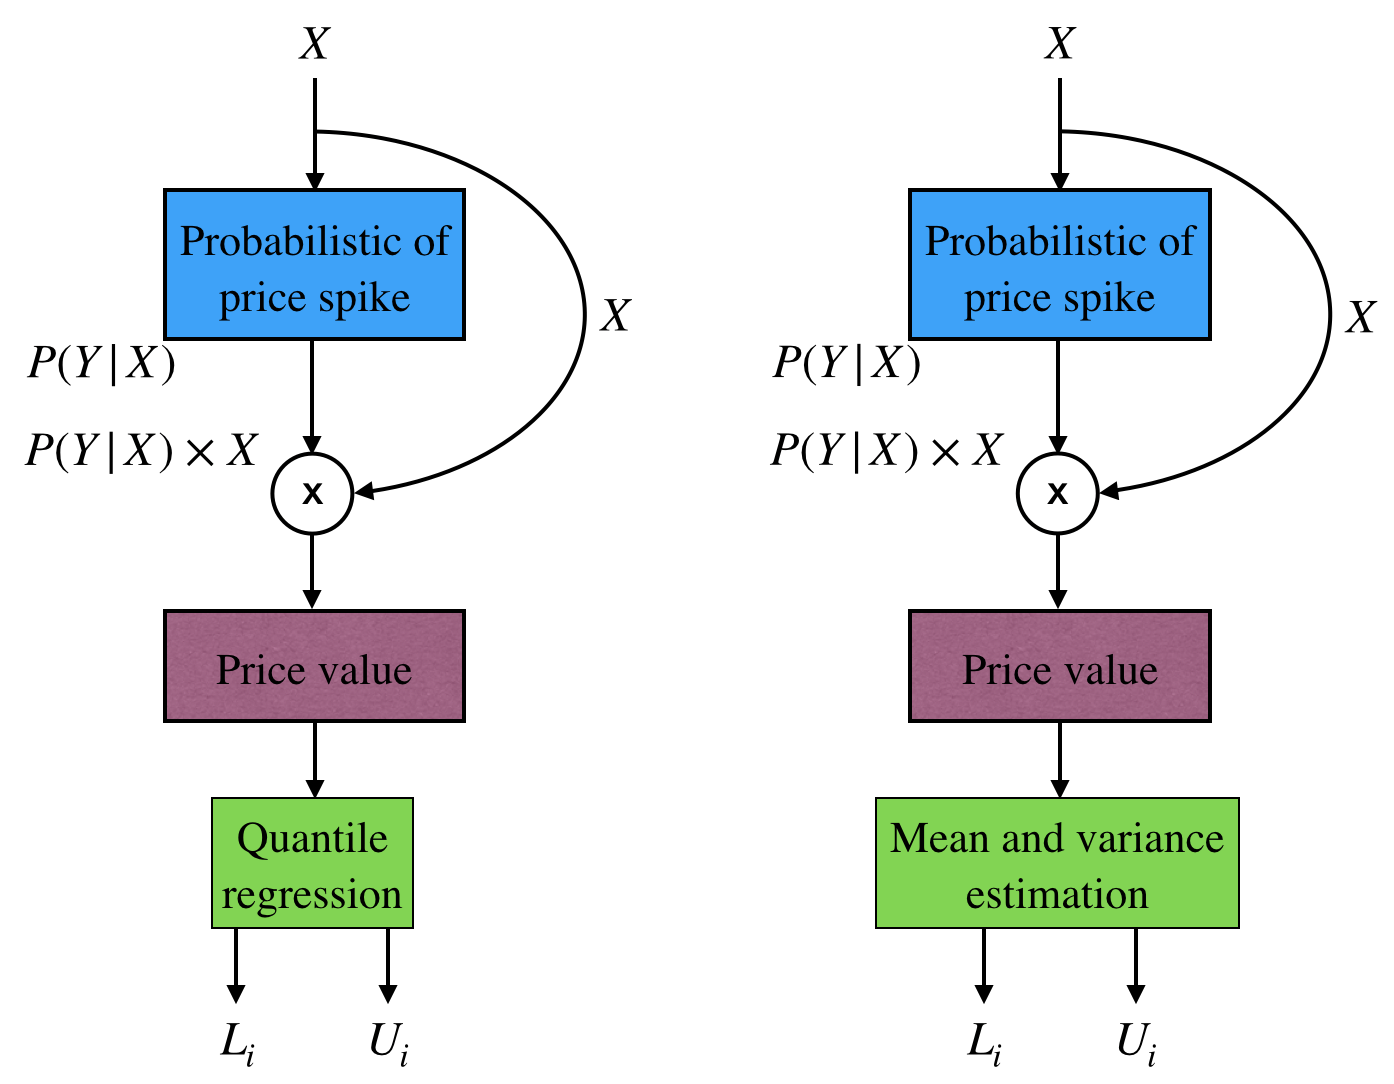
\includegraphics[width=12cm]{UB_LB_MV_PDRNN}
        \caption{Upper and lower bound and mean-variance estimation}
        \label{Fig:UB_LB_MV_PDRNN}
        \centering
      \end{figure}

    \subsection{Evaluation metrics}
      This section will descrip evaluation metrics in accuracy and reliable point of view.
      In term of accuracy metric, the forecasting results will be analyzied using pinball function.
      The Coverage Width-baed Criterion (CWC) will take care of reliability point of view.

      \subsubsection{Accuracy}
        The widely used measurement of forecasting's accuracy is mean absoulute error (MAE) which is simply and generalized method.
        MAE work well of point of forecasting (single value).
        However, this problem is to formulate upper and lower bound of forecasting which is cooperated with confidence value.
        Hence, general MAE is not satisfied in this case.
        Pinball loss function are proposed in \cite{Maciejowska2016}, also be benchmark of this paper, which returns the value that can be interpreted as accuracy of mean-varience and quantile regression forecasting models.
        The pinball loss function is formulated as below.

        \begin{equation}
          L_{\tau}(y,z) =
          \begin{cases}
            (y-z)\tau if y>=z \\
            (z-y)(1-\tau) if z>y
          \end{cases}
          \label{eq.pinball}
        \end{equation}
        where $L_{\tau}(y,z)$ is pinball loss function at $\tau$ confidence level, $y$ is forecasted electricity price and $z$ is actual electricty price.
        The final score of pinball loss function was computed as average $L_{\tau}$ across 24 hours for each task.
        The $\tau$ in this paper is 0.05, 0.10, 0.15, 0.20 and 0.25 which are represent 5$\%$, 10$\%$, 15$\%$, 20$\%$ and 25$\%$ confidence levels.
        The important results of pinball loss function is that the lower pinball loss, the more accurate forecasting model.

      \subsubsection{Reliability}
        In term of reliability measurement, the performance of forecasting model is measured to ensure that the ranges of forecasting can cover the observation values both quality and quantity.
        First,  PI converage probility (PICP) refers to the ability of the constructed PIs to capture the actual target variables.
        PICP can be methematically stated as
        \begin{equation}
          PICP = \frac{1}{N} \sum_{i=1}^{N} C_{i}
          \label{eq.PICP}
        \end{equation}
        where
        \begin{equation}
          C_{i} =
          \begin{cases}
            1, if t_{i} \in [L_{i},U_{i}] \\
            0, if t_{i} \not\in [L_{i},U_{i}]
          \end{cases}
          \label{eq.Ci}
        \end{equation}

        where $N$ is the number of samples in the test set, $t_{i}$ represents the actual target, and $L_{i}$ and $U_{i}$ are lower and upper bounds of hte $i$th PI, repestively.
        The range of PICP lies between 0$\%$ (wher none of hte targets are enclosed by PI) to 100$\%$ (when all targets are enclosed by PI).
        Ideally, PICP should be very close or larger than the norminal confidence level associated to the PIs.
        PICP has a direct relationship with the width of PIs.
        A satisfactorily large PICP can be easily achieved by widening PIs from either side.
        However, such PIs are too conservative and less useful in practice, as they do not show the variation of the targetes.
        Therefore, a measure is resquired to check how wide the PIs are.
        Mean PI Width (MPIW) quantifies this aspect of PIs \cite{Khosravi2010}.

        \begin{equation}
          MPIW = \frac{1}{N} \sum_{i=1}^{N} (U_{i}-L_{i})
          \label{eq.MPIW}
        \end{equation}

        Secondrly, MPIW shows the average width of PIs.
        Normalizing MPIW by the range of the underlying target, $R$, allows us to compare PIs constructed for different datasets repectively (the new measure is called NMPIW),
        \begin{equation}
          NMPIW = \frac{NMPIW}{R}
          \label{eq.NMPIW}
        \end{equation}

        Both PICP and NMPIW, are representing quality and width of PIs, evaluate the quality of PIS from one aspect.
        A combined index is required for the comprehensive assessment of PIs from both coverage probility and width perspectives.
        The new measure should give a higher priority to PICP, as it is the key feature of PIs determining whether constructed PIs are theoretically correcty or not.
        The Coverage Width-baed Criterion (CWC) evalutes PIs from both coverage probility and width perspectives.

        Where, $\eta$ and $\mu$ are two hyperparameters controlling the location and amount of CWC jump.
        These measures can be easily determined based on the level of confidence associated with PIs.
        $\mu$ correspomds to the nominal confidence level associated with PIs and can be set to 1-$\alpha$.
        The design of CWC is based on two principles:

        \begin{itemize}
          \item if PICP is less than the nominal confidence level, (1-$\alpha$)$\%$, CWC should be large regardless of the width of PIs (measures by NMIPW),
          \item if PICP is greater than or equal to its corresponding confidence level, then NMPIW should be the influential factor.
          $\gamma$(PICP), eliminates the exponential term of CWC when PICP is greater or equal to the nominal confidence level.
        \end{itemize}

    \subsection{Data description}
      All data in this paper is provided in Global Energy Forecasting Competition 2014 (see \cite{Hong2016}).
      The aim of this competition is to forecast 15 tasks of electricity prices in term of probabilistic distribution (in quantiles).
      Hourly data of locational marginal price (LMP), zonal load forecast and system load forecast are provided.
      The participants receive historical data and forecast for next day electricty price.
      In total, the price forecasting track involves about three years of locational marginal price, zonal and system load forecast.
      The summarized solution data set of 15 tasks is shown in table~\ref{table:price_data_set}.

      \begin{table}[H]
        \begin{center}
        \caption{GEFCom2014 task solution}
        \begin{adjustbox}{width=\textwidth}
          \begin{tabular}{|c|c|c|c|c|c|c|}
            \hline
            Task & Day & Holiday & Season & Normal price & High price & Spike price\\
            \hline
            1 & Sun & Yes & Summer & 24 & - & -\\
            2 & Mon & No & Summer & 24 & - & -\\
            3 & Mon & No & Summer & 22 & 2 & -\\
            4 & Thu & No & Summer & 24 & - & -\\
            5 & Tue & No & Summer & 22 & 2 & -\\
            6 & Sat & Yes & Summer & 24 & - & -\\
            7 & Tue & No & Summer & 16 & 8 & -\\
            8 & Thu & No & Summer & 12 & 8 & 4\\
            9 & Fri & No & Summer & 13 & 6 & 5\\
            10 & Sat & Yes & Summer & 18 & 6 & -\\
            11 & Wed & No & Summer & 24 & - & -\\
            12 & Thu & No & Summer & 24 & - & -\\
            13 & Sat & Yes & Authumn & 24 & - & -\\
            14 & Sun & Yes & Authumn & 24 & - & -\\
            15 & Tue & No & Authumn & 15 & 9 & -\\
            \hline
          \end{tabular}
        \end{adjustbox}
        \label{table:price_data_set}
        \end{center}
      \end{table}

      The participation teams in GEFCom2014 perform electricity price forecasting method i.e.; linear regression (IR)\cite{Dudek2016}, multilayer perceptron (MLP)\cite{Dudek2016},  multiple quantile regression\cite{Juban2016}, hybrid quantile estimation with pre-and-post processes\cite{Maciejowska2016}.
      These data are fed into the proposed MLP and Deep ResNet models during training section with the Levenberg-Marquardt algorithm to provent overfitting problems.
  \section{Results}
    What is comparision? benchmark is provided from GEFCom2014, task4-\cite{Dudek2016}, \cite{Maciejowska2016}, \cite{Khosravi2011}

    The proposed Deep ResNet generates upper and lower bound values using quantile regression and mean-varience method.
    In accuracy point of view, the results are summarized in ~\ref{table:result_pinball}.

    \begin{table}[H]
      \caption{The results of probabilistic electricity price forecasting compared to benchmarks}
      \begin{adjustbox}{width=\textwidth}
      \begin{threeparttable}
        \begin{center}
          \begin{tabular}{ccccccccccccc}
            \hline
            Method & Task 4 & Task 5& Task 6 & Task 7& Task 8 & Task 9& Task 10 & Task 11& Task 12 & Task 13 & Task 14 & Task 15\\
            \hline
            Benchmark 1 \tnote{a} & 4.03 & 7.97 & 5.70 & 22.32 & 38.34 & 44.23 & 18.22 & 31.57 & 42.95 & 2.86 & 3.20 & 22.38\\
            Benchmark 2 \tnote{b} & 1.00 & 1.82 & 1.19 & 2.82 & 7.56 & 4.21 & 2.60 & 1.05 & 1.24 & 4.06 & 1.08 & 3.07 \\
            \hline
            MLP-MV & 4.19 & 4.33 & 4.18 & 10.48 & 31.57 & 33.35 & 6.28 & 4.28 & 4.25 & 4.06 & 4.05 & 13.02\\
            MLP-QR & 2.57 & 4.03 & 2.55 & 12.96 & 34.76 & 36.24 & 8.83 & 2.51 & 2.49 & 2.47 & 2.62 & 16.81\\
            Deep ResNet-MV& 2.45 & 3.36 & 2.39 & 5.79 & 8.79 & 6.95 & 5.80 & 2.41 & 2.41 & 2.34 & 2.43 & 11.02 \\
            Deep ResNet-QR& 2.11& 3.47& 1.93 & 6.14 & 9.41 & 7.63 & 6.38 & 1.88 & 1.91 & 2.01 & 2.22 &11.70 \\
            \hline
          \end{tabular}
          \begin{tablenotes}
            Notes: The numbers are calculated according to the pinball function
            \item[a] provided by GEFCom2014
            \item[b] provided in \cite{Maciejowska2016}.
          \end{tablenotes}
          \end{center}
      \end{threeparttable}
      \end{adjustbox}
      \label{table:result_pinball}
    \end{table}

    The figure~\ref{Fig:CWC} illustrates the reliability perspective of MLP and Deep ResNet models.
    The CWC values are average values of task 1 to 15.
    \begin{figure}[H]
      \centering
      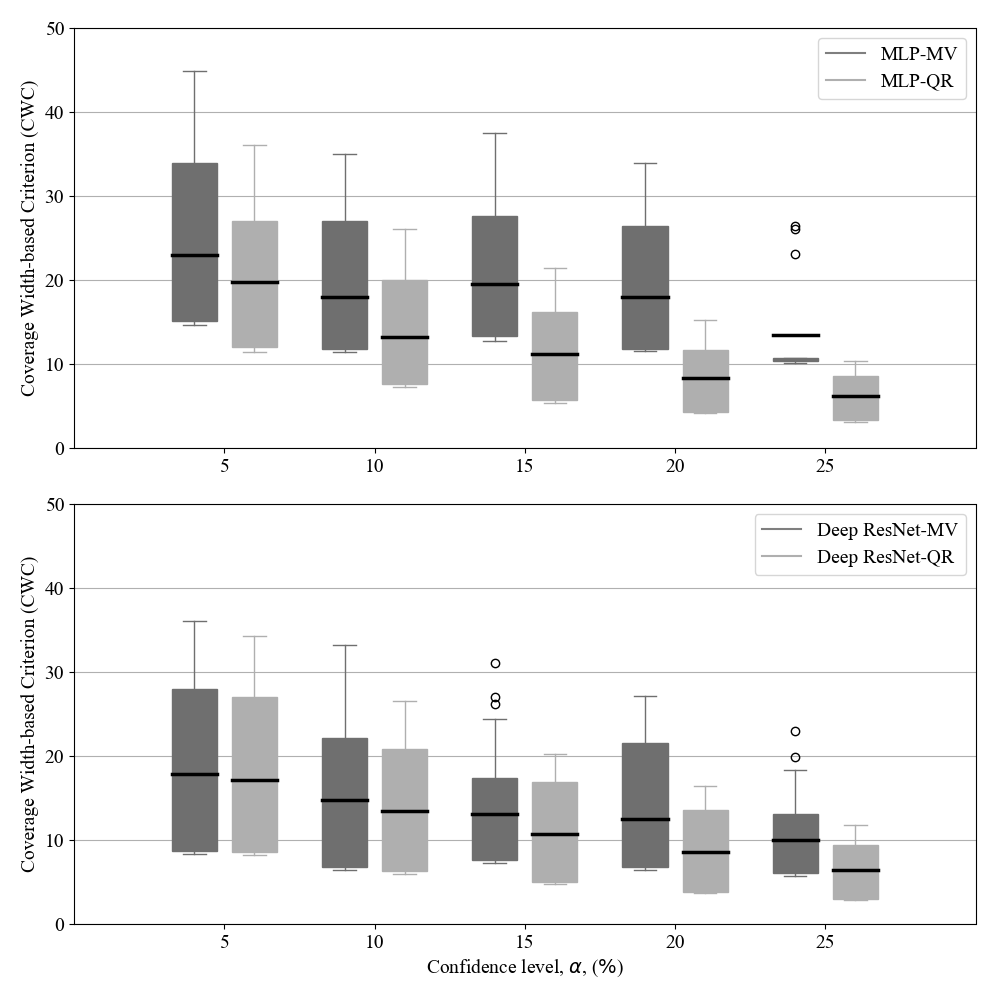
\includegraphics[width=12cm]{boxcompare_MV-QR}
      \caption{The results of reliability aspect are represented in CWC values.
      The CWC values of MLP and Deep ResNet methods with difference confidence level are shown in upper and lower figure, respectively}
      \label{Fig:CWC}
    \end{figure}
    The results of the proposed MLP and Deep ResNet models using quantile regression are illustrated on Task 9.
    In Figure~\ref{Fig:compare_spike_and_non_spike_model}, the filled area represent interval prediction of MLP-QR and Deep ResNet-QR with 5$\%$ confidence level.
    In this task 9, Deep ResNet-QR can handle high price and spike price in observation values where MLP could not handle it.
    Consequently, the proposed Deep ResNet could imporve reliability of forecasting model.
    \begin{figure}[H]
      \centering
      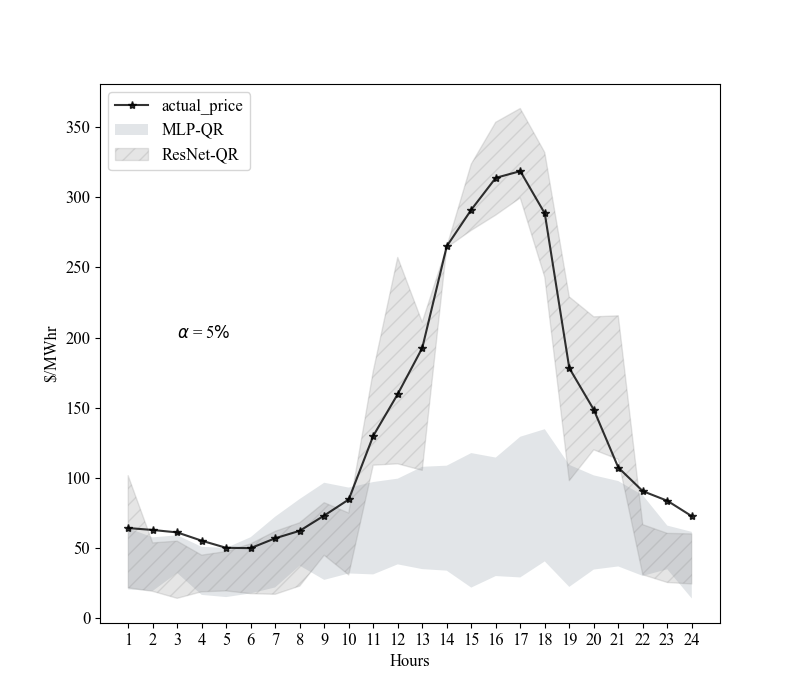
\includegraphics[width=12cm]{Task_9-compare_between_non-spike_and_spike}
      \caption{The results of MLP (non-spike price detection) model and Deep ResNet (spike price prediction) model with quantile regression method on confidence level ($\alpha$ = 5$\%$ on Task 9}
      \label{Fig:compare_spike_and_non_spike_model}
    \end{figure}

    \begin{figure}[H]
      \centering
      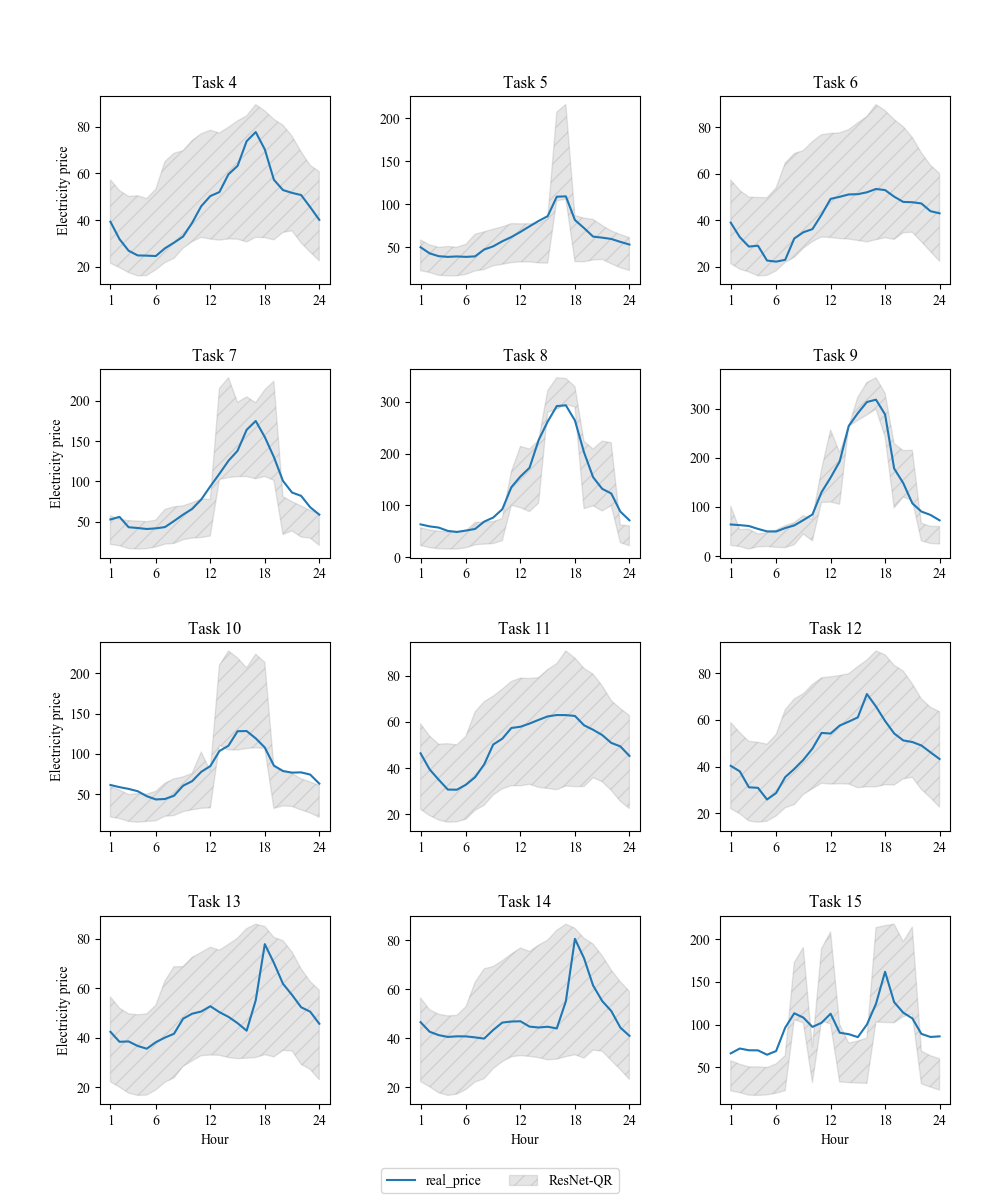
\includegraphics[width=15cm]{All_task_with_spike_price_QR_005}
      \caption{All task with Deep ResNet-QR with 5$\%$ confidence level}
      \label{Fig:all_task_QR_005}
    \end{figure}

  \section{Conclusions}
    This paper proposes a novel application of Deep Residual Neural Network (Deep ResNet) based approach to probabilistic electricity price forecasting in term of quaintile regression and mean-varience estimation. The two significatant observation results were: (i)
  \section*{References}
  \bibliography{mybibfile}
\end{document}
